\begin{frame}[shrink=15]
  \frametitle{Equations of motion}
  \begin{block}{}
    \begin{equation*}
      B(\vec{q}) \ddot{\vec{q}} + C(\vec{q}, \dot{\vec{q}}) \dot{\vec{q}} + \cancel{\vec{G}(\vec{q})} = \vec{\tau} - {}^{b}J^{T}_{F} {}^b\vec{w}_{F} 
      \longrightarrow {}^{ws}\ddot{\vec{x}} = \vec{a}
    \end{equation*}
    \begin{equation*}
      \vec{q} = 
      \begin{bmatrix}
        q_1 & q_2 & q_3 & q_4 & q_5 & q_6 & q_7
      \end{bmatrix}^T
      \quad
          {}^{ws}\vec{x} = 
          \begin{bmatrix}
            r_x & r_y & r_z & \psi & \theta & \phi
          \end{bmatrix}^T
    \end{equation*}
    \begin{equation*}
      {}^{ws}R_{ee} = R_{ZYX}(\psi, \theta, \phi) = R_{ZYX}(\vec{\Phi})
    \end{equation*}
  \end{block}

  \vskip-1em
  \begin{columns}[t]
    \begin{column}{0.4\textwidth}
      \begin{itemize}
      \item<2->[] Joint Space description
      \item<2->[] $\vec{\tau} = C \dot{\vec{q}} + {}^{b}J^{T}_{F} ({}^b\vec{\gamma} + {}^b\vec{w}_{F})$
      \item<3->[] $\ddot{\vec{q}} = B^{-1} ({}^{b}J^{T}_{F}) {}^b\vec{\gamma}$
      \end{itemize}
    \end{column}
    \begin{column}{0.8\textwidth}
      \begin{itemize}
      \item<4->[] HIC requires operational space description
      \item<4->[] ${}^{ws} \ddot{\vec{x}} = {}^{ws} J_{A,E} \ddot{\vec{q}} + {}^{ws} \dot{J_{A,E}} \dot{\vec{q}}$
      \item<5->[] ${}^{ws} J_{A,E} = 
        \left[
          \begin{smallmatrix}
            I & 0 \\
            0 & T^{-1}(\vec{\Phi})
          \end{smallmatrix}
          \right]$
        ${}^{ws} J_{E} \quad {}^{ws}\vec{\omega} = T(\vec{\Phi}) \vec{\dot{\Phi}}$\\
        $\mathrm{det}(T) = -\cos(\theta) \neq 0$\\
        ${}^{ws} \dot{J_{A,E}} = 
        \left[
          \begin{smallmatrix}
            0 & 0 \\
            0 & -T^{-1} \dot{T} T^{-1}
          \end{smallmatrix}
          \right]
             {}^{ws} J_{E} + 
             \left[
               \begin{smallmatrix}
                 I & 0 \\
                 0 & T^{-1}
               \end{smallmatrix}
               \right]
                  {}^{ws} \dot{J}_{E}$
      \end{itemize}
    \end{column}
  \end{columns}
  \begin{columns}
    \begin{column}{2\textwidth}
      \begin{itemize}
      \item<6->[]Substitute $\ddot{\vec{q}}$ in the operational space description
      \item<6->[]${}^{ws} \ddot{\vec{x}} = \underbrace{{}^{ws} J_{A,E} B^{-1} ({}^b J_{F}^T)}_{B_A^{-1}} {}^b \vec{\gamma} + {}^{ws} \ddot{J_{A,E}} \dot{\vec{q}}$
      \item<7->[]$B_A {}^{ws} \ddot{\vec{x}} =  \vec{\gamma} +  B_A  {}^{ws} \dot{J_{A,E}} \dot{\vec{q}}$
      \item<8->[]$\vec{\gamma} = B_A \vec{a} - B_A {}^{ws} \dot{J_{A,E}} \dot{\vec{q}}$
      \item<9->[]$\vec{\tau} = C \dot{\vec{q}} + {}^{b}J^{T}_{F} ( B_A \vec{a} - B_A {}^{ws} \dot{J_{A,E}} \dot{\vec{q}} + {}^b\vec{w}_{F})
        \Longrightarrow {}^{ws}\ddot{\vec{x}} = \vec{a} $
      \end{itemize}
    \end{column}
  \end{columns}
\end{frame}

\begin{frame}
  \frametitle{Hybrid Impedance control}
  \framesubtitle{Control problem statement}
  Given ${}^{ws}\ddot{\vec{x}} = \vec{a} $ find $\vec{a}$ such that
  \begin{itemize}
  \item[-]$r_x$ and $r_y$ are position/impedance controlled i.e.
    \begin{itemize}
    \item[-] $\ddot{e}_{x} + B_x \dot{e}_x + K_x e_x = {}^{ws}F_x$
    \item[-] $\ddot{e}_{y} + B_y \dot{e}_y + K_y e_y = {}^{ws}F_y$
    \end{itemize}
  \item[-]the attitude of the end effector is rigidly controlled i.e.
    \begin{itemize}
    \item[-] $\ddot{\vec{e}}_{\Phi} + B_{\Phi} \dot{\vec{e}}_{\Phi} + K_{\Phi} \vec{e}_{\Phi} = \vec{0}$
    \end{itemize}
  \item[-]$r_z$ is force controlled i.e.
    \begin{itemize}
    \item[-] $e_z \xrightarrow[t \to \infty]{} 0$
    \end{itemize}
  \end{itemize}
\end{frame}

\begin{frame}
  \frametitle{Hybrid Impedance control}
  \framesubtitle{Modelling the environment}
  \centering
  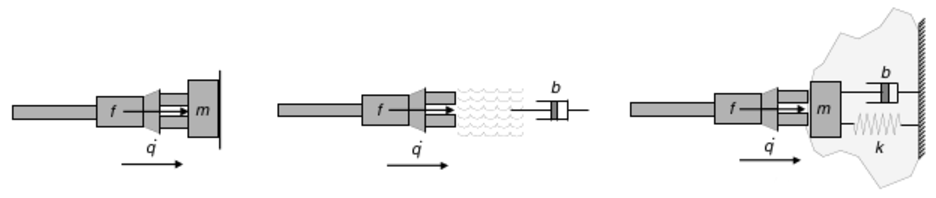
\includegraphics[scale=0.75]{type_of_impedances}
  \begin{itemize}
  \item[-] for each DoF the manipulator and the environment can be described using impedances $Z_m$ and $Z_e$
  \item[-] the environment is defined to be any element connected to or contacting the robot anywhere \textcolor{red}{\emph{past the wrist}} force sensor
  \item[-] $Z(\omega) = R(\omega) + j X(\omega)$
  \item[-] type of impedances
    \begin{itemize}
    \item[] inertial iff $|Z(0)| = 0$
    \item[] resistive iff $|Z(0)| = c \in (0, \infty)$
    \item[] capacitive iff $|Z(0)| = \infty$
    \end{itemize}
  \end{itemize}
\end{frame}

\begin{frame}
  \frametitle{Hybrid Impedance control}
  \framesubtitle{Duality principle for position control}
  Manipulator impedance chosen as the dual of the environment impedance
  \begin{columns}
    \begin{column}{0.5\columnwidth}
      \begin{flalign*}
        &v = \frac{Z_m(s)}{Z_m(s) + Z_e(s)}v_{des} - \frac{F_{env}}{Z_e + Z_m} &\\
      \end{flalign*}
    \end{column}
    \begin{column}{0.5\columnwidth}
      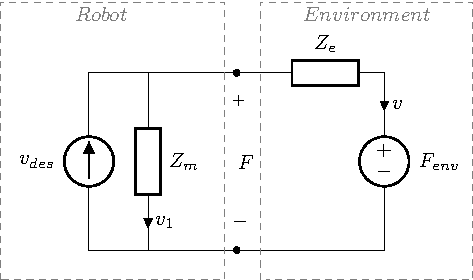
\includegraphics[width=\columnwidth]{position_control_model}
    \end{column}
  \end{columns}
  \begin{equation*}
    &e_{ss} \Big|_{F_{env}(t) \equiv 0} = \lim_{s \to 0}(v - v_{des}) = \frac{-Z_e(0)}{Z_m(0) + Z_e(0)} = 0 \text{ as long as } Z_m(0) \neq 0&
  \end{equation*}
  \begin{block}{Rule of thumb}
    inertial environments are position controlled with a noninertial manipulator impedances
  \end{block}
\end{frame}

\begin{frame}[shrink=10]
  \frametitle{Hybrid Impedance control}
  \framesubtitle{Position-Controlled subsystem}
  \begin{columns}
    \begin{column}{0.4\textwidth}
      \begin{align*}
        &v_{des} = v + v_1\\
        &v_1 = \frac{F}{Z_m}\\ 
        &F = Z_e v + F_{env}\\
        &a = \dot{v} = \frac{\mathrm{d}}{\mathrm{d}t} \left(v_{des} - \frac{F}{Z_m} \right)\\
        &Z_m = M s + \tilde{Z}_m\\
      \end{align*}
    \end{column}
    \begin{column}{0.5\textwidth}
      \centering
      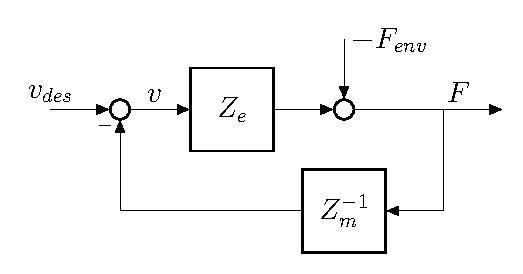
\includegraphics[scale=0.8]{position_control_feedback}
    \end{column}
  \end{columns}

  \begin{align*}
    &a = \frac{\mathrm{d}}{\mathrm{d}t} \left(v_{des} - \frac{F}{Ms + \tilde{Z}_m} \right) = \dot{v}_{des} - \frac{Fs}{Ms + \tilde{Z}_{m}} = \dot{v}_{des} - s v_1 \\
    &F = v_1 (Ms + \tilde{Z}_m) \quad v_1 = \frac{F - (v_{des} - v)\tilde{Z}_m}{Ms}\\
    &a = \dot{v}_{des} - s v_1 = \dot{v}_{des} - \cancel{s} \left( \frac{F - (v_{des} - v)\tilde{Z}_m}{M\cancel{s}} \right) = \dot{v}_{des} + \frac{(v_{des} - v)\tilde{Z}_m}{M} - \frac{F}{M}
  \end{align*}
\end{frame}

\begin{frame}
  \frametitle{Hybrid Impedance control}
  \framesubtitle{Duality principle for force control}
  Manipulator impedance chosen as the dual of the environment impedance
  \begin{columns}
    \begin{column}{0.5\columnwidth}
      \begin{flalign*}
        F = \frac{Z_e(s)}{Z_m(s) + Z_e(s)}F_{des} + \frac{Z_e Z_m}{Z_m + Z_e} V_{env}
      \end{flalign*}
    \end{column}
    \begin{column}{0.45\columnwidth}
      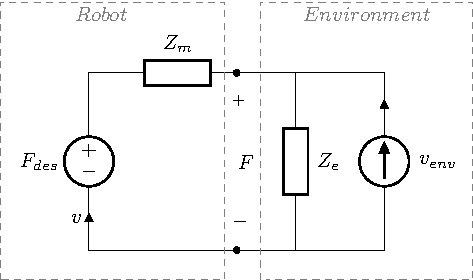
\includegraphics[width=\columnwidth]{force_control_model}
    \end{column}
  \end{columns}
  \begin{equation*}
    e_{ss} \Big|_{v_{env}(t) \equiv 0} = \lim_{s \to 0}(F - F_{des}) = \frac{-Z_m(0)}{Z_m(0) + Z_e(0)} = 0 \text{ as long as } Z_m(0) < \infty
  \end{equation*}
  \begin{block}{Rule of thumb}
    capacitive environments are force controlled with noncapacitive manipulator impedances
  \end{block}
\end{frame}

\begin{frame}[shrink=10]
  \frametitle{Hybrid Impedance control}
  \framesubtitle{Force-Controlled subsystem}
  \begin{columns}
    \begin{column}{0.4\textwidth}
      \begin{align*}
        &F = F_{des} + Z_m v\\
        &v = \frac{F - F_{des}}{Z_m}\\
        &F = Z_e(v + v_{env})\\
        &a = \dot{v} = \frac{\mathrm{d}}{\mathrm{d}t} \left(\frac{F - F_{des}}{Z_m} \right)\\
        &Z_m = M s + \tilde{Z}_m\\
      \end{align*}
    \end{column}
    \begin{column}{0.5\textwidth}
      \centering
      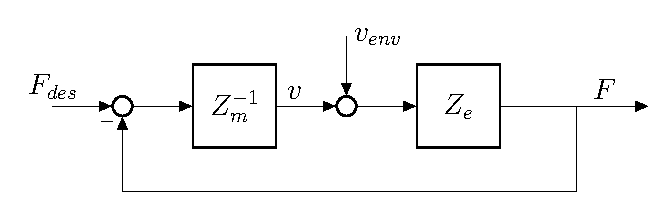
\includegraphics[scale=0.8]{force_control_feedback}
    \end{column}
  \end{columns}

  \begin{align*}
    &a = \frac{\mathrm{d}}{\mathrm{d}t} \left(\frac{F - F_{des}}{Ms + \tilde{Z}_m} \right) = \left(\frac{s(F - F_{des})}{Ms + \tilde{Z}_m} \right)\\
    &vMs + v \tilde{Z}_m = F - F_{des}\\
    &v = \frac{1}{Ms} (F - F_{des} - v \tilde{Z}_m )\\
    &a = \dot{v} = \frac{\cancel{s}}{M\cancel{s}} (F - F_{des}) - \frac{\cancel{s}}{M\cancel{s}}( \tilde{Z}_m v) = \frac{1}{M} (F - F_{des}) - \frac{1}{M}( \tilde{Z}_m v) \\
  \end{align*}
\end{frame}

\begin{frame}
  \frametitle{Hybrid Impedance control}
  \framesubtitle{Control assigned to each DoF}
  Position (${}^{ws}r_x,{}^{ws}r_y$):
  \begin{itemize}
  \item[-] inertial environment (manipulator moving a payload along given axis)
  \item[-] $Z_{m,p} = M_p s + \tilde{Z}_{m,p} = M_p s + B_p + \frac{K_p}{s}$
  \item[-] $a_{p} = a_{des,p} + \frac{B_p}{M_p} (v_{des,p} - v_p) + \frac{K_p}{M_p} (x_{des,p} - x_p) - \frac{F_p}{M_p}$
  \end{itemize}
  Attitude ($\psi$, $\theta$, $\phi$):
  \begin{itemize}
  \item[-] inertial environment (manipulator rotating a payload about given axis )
  \item[-] $Z_{m,a} = M_a s + \tilde{Z}_{m,a} = M_a s + B_a + \frac{K_a}{s}$
  \item[-] $a_a = a_{des,a} + \frac{B_a}{M_a} (v_{des,a} - v_a) + \frac{K_a}{M_a} (x_{des,a} - x_a)$
  \end{itemize}
  Force (${}^{ws}f_z$):
  \begin{itemize}
  \item[-] capacitive environment
  \item[-] $Z_{m,f} = M_f s + \tilde{Z}_{m,f} = M_f s + B_f$
  \item[-] $a_{f} = M_f^{-1}((f_{des} - f) - B_f v_z)$
  \end{itemize}  
\end{frame}

\begin{frame}
  \frametitle{Hybrid Impedance control}
  \framesubtitle{Filtering action}
  In principle one could assign a position control law \textcolor{red}{\emph{and}} a force
  control law for \textcolor{red}{\emph{each}} DoF
  
  A selection matrix $S$ is used to separate the force-controlled and position-controlled \emph{reciprocal} subspaces
  \begin{columns}
    \begin{column}{0.6\textwidth}
      \begin{flalign*}
        &\vec{a}_p = 
        \begin{bmatrix}
          a_{p,x} & a_{p,y} & a_{p,z}
        \end{bmatrix}^T&\\
        &\vec{a}_a = 
        \begin{bmatrix}
          a_{a, \psi} & a_{a, \theta} & a_{a, \phi}
        \end{bmatrix}^T&\\
        &\vec{a}_f = 
        \begin{bmatrix}
          a_{f,x} & a_{f,y} & a_{f,z} & a_{f, \psi} & a_{f, \theta} & a_{f, \phi}
        \end{bmatrix}^T&\\
        &\vec{a} = S 
        \begin{bmatrix}
          \vec{a}_p \\
          \vec{a}_a
        \end{bmatrix} + (I - S) \vec{a}_f&
      \end{flalign*}
    \end{column}
    \begin{column}{0.35\columnwidth}
      $
      S =
        \begin {bmatrix}
          1 & 0 & 0 & 0 & 0 & 0\\
          0 & 1 & 0 & 0 & 0 & 0\\
          0 & 0 & 0 & 0 & 0 & 0\\
          0 & 0 & 0 & 1 & 0 & 0\\
          0 & 0 & 0 & 0 & 1 & 0\\
          0 & 0 & 0 & 0 & 0 & 1\\
        \end {bmatrix}
      $
    \end{column}
  \end{columns}
\end{frame}

\begin{frame}
  \frametitle{Hybrid Impedance control}
  The resulting control law is
  \begin{align*}
    & a_x = \ddot{r}_{x,des} + B_x (\dot{r}_{x,des} - \dot{r}_x) + K_x (r_{x,des} - r_x) - F_x \\
    & a_y = \ddot{r}_{y,des} + B_y (\dot{r}_{y,des} - \dot{r}_y) + K_y (r_{y,des} - r_y) - F_y \\
    & a_z = - B_f \dot{r}_z + K_f(F_{z,des} - F_z) \\
    & a_{\psi} = \ddot{\psi}_{des} + B_{\psi}(\dot{\psi}_{des} - \dot{\psi}) + K_{\psi} (\psi_{des} - \psi) \\
    & a_{\theta} = \ddot{\theta}_{des} + B_{\theta}(\dot{\theta}_{des} - \dot{\theta}) + K_{\theta} (\theta_{des} - \theta) \\
    & a_{\phi} = \ddot{\phi}_{des} + B_{\phi}(\dot{\phi}_{des} - \dot{\phi}) + K_{\phi} (\phi_{des} - \phi) \\
  \end{align*}
\end{frame}
